\section{Background}
Censorship resistance~\cite{DBLP:conf/ccs/KelkarDLJK23,DBLP:conf/nsdi/YangPAKT22,DBLP:journals/corr/abs-2307-10185} is an important feature of decentralized systems,
missing from many state-of-the-art and even deployed consensus protocols.
In leader-based protocols the leader arbitrarily selects the transactions to be included in the new block,
% In a model where at most $f$ of the $n$ replicas can be malicious, the adversary can delay honest transactions by $f$ blocks.
and so does a block builder in permissionless protocols, such as Bitcoin and Ethereum.
Multiple solutions have been proposed.
One approach employs multiple parallel leaders~\cite{DBLP:journals/corr/abs-1906-05552,DBLP:conf/sirocco/AvarikiotiHSVWW23, DBLP:conf/nsdi/YangPAKT22,DBLP:journals/corr/abs-2307-10185,DBLP:conf/ccs/MillerXCSS16,DBLP:conf/eurosys/DanezisKSS22}, which inevitably leads to duplication of transactions in the output of the protocol.
Other solutions employ cryptography~\cite{DBLP:conf/ccs/MillerXCSS16, DBLP:conf/aft/ZhangMQBEF23, DBLP:conf/crypto/CachinKPS01,Malkhi2022MaximalEV}, such as threshold or time-based encryption, which sacrifice efficiency.

In a different line of work, recent literature has recognized the redundancy of consensus for implementing asset-transfer systems~\cite{DBLP:journals/dc/GuerraouiKMPS22}.
Such schemes have been described in theory~\cite{DBLP:journals/corr/abs-1909-10926, DBLP:conf/dsn/CollinsGKKMPPST20} and deployed in the real world~\cite{DBLP:conf/aft/BaudetDS20}.
Yet, the proposed protocols are tailor-made for payment systems or for specific blockchains and cannot  be used for arbitrary distributed applications.

The goal of this project is to further design and develop \emph{Partially Ordered Dataset (POD)},
a solution that allows censorship-resistant recording of arbitrary messages.
POD can be used as the base for a wide range of consensus-less applications,
such as payment systems,
a shared mempool layer for decentralized sequencers,
auctions with non-omission guarantees, and storing feeds for decentralized social media.
By giving up on total order we result in a high-performant layer in terms of both throughput and latency.

\section{The project}
POD associates messages (which we refer to as \emph{transactions}, as common in the literature) with \emph{timestamps}.
It does not guarantee full ordering, as classical consensus mechanisms do, but instead results in a `fluctuating order'.
That is, honest users may observe different timestamps for each transaction, yet the timestamps will be within a restricted and well-defined interval.
% and users will agree on the set of observed transactions.

\begin{minipage}{.45\textwidth}
    \begin{center}
      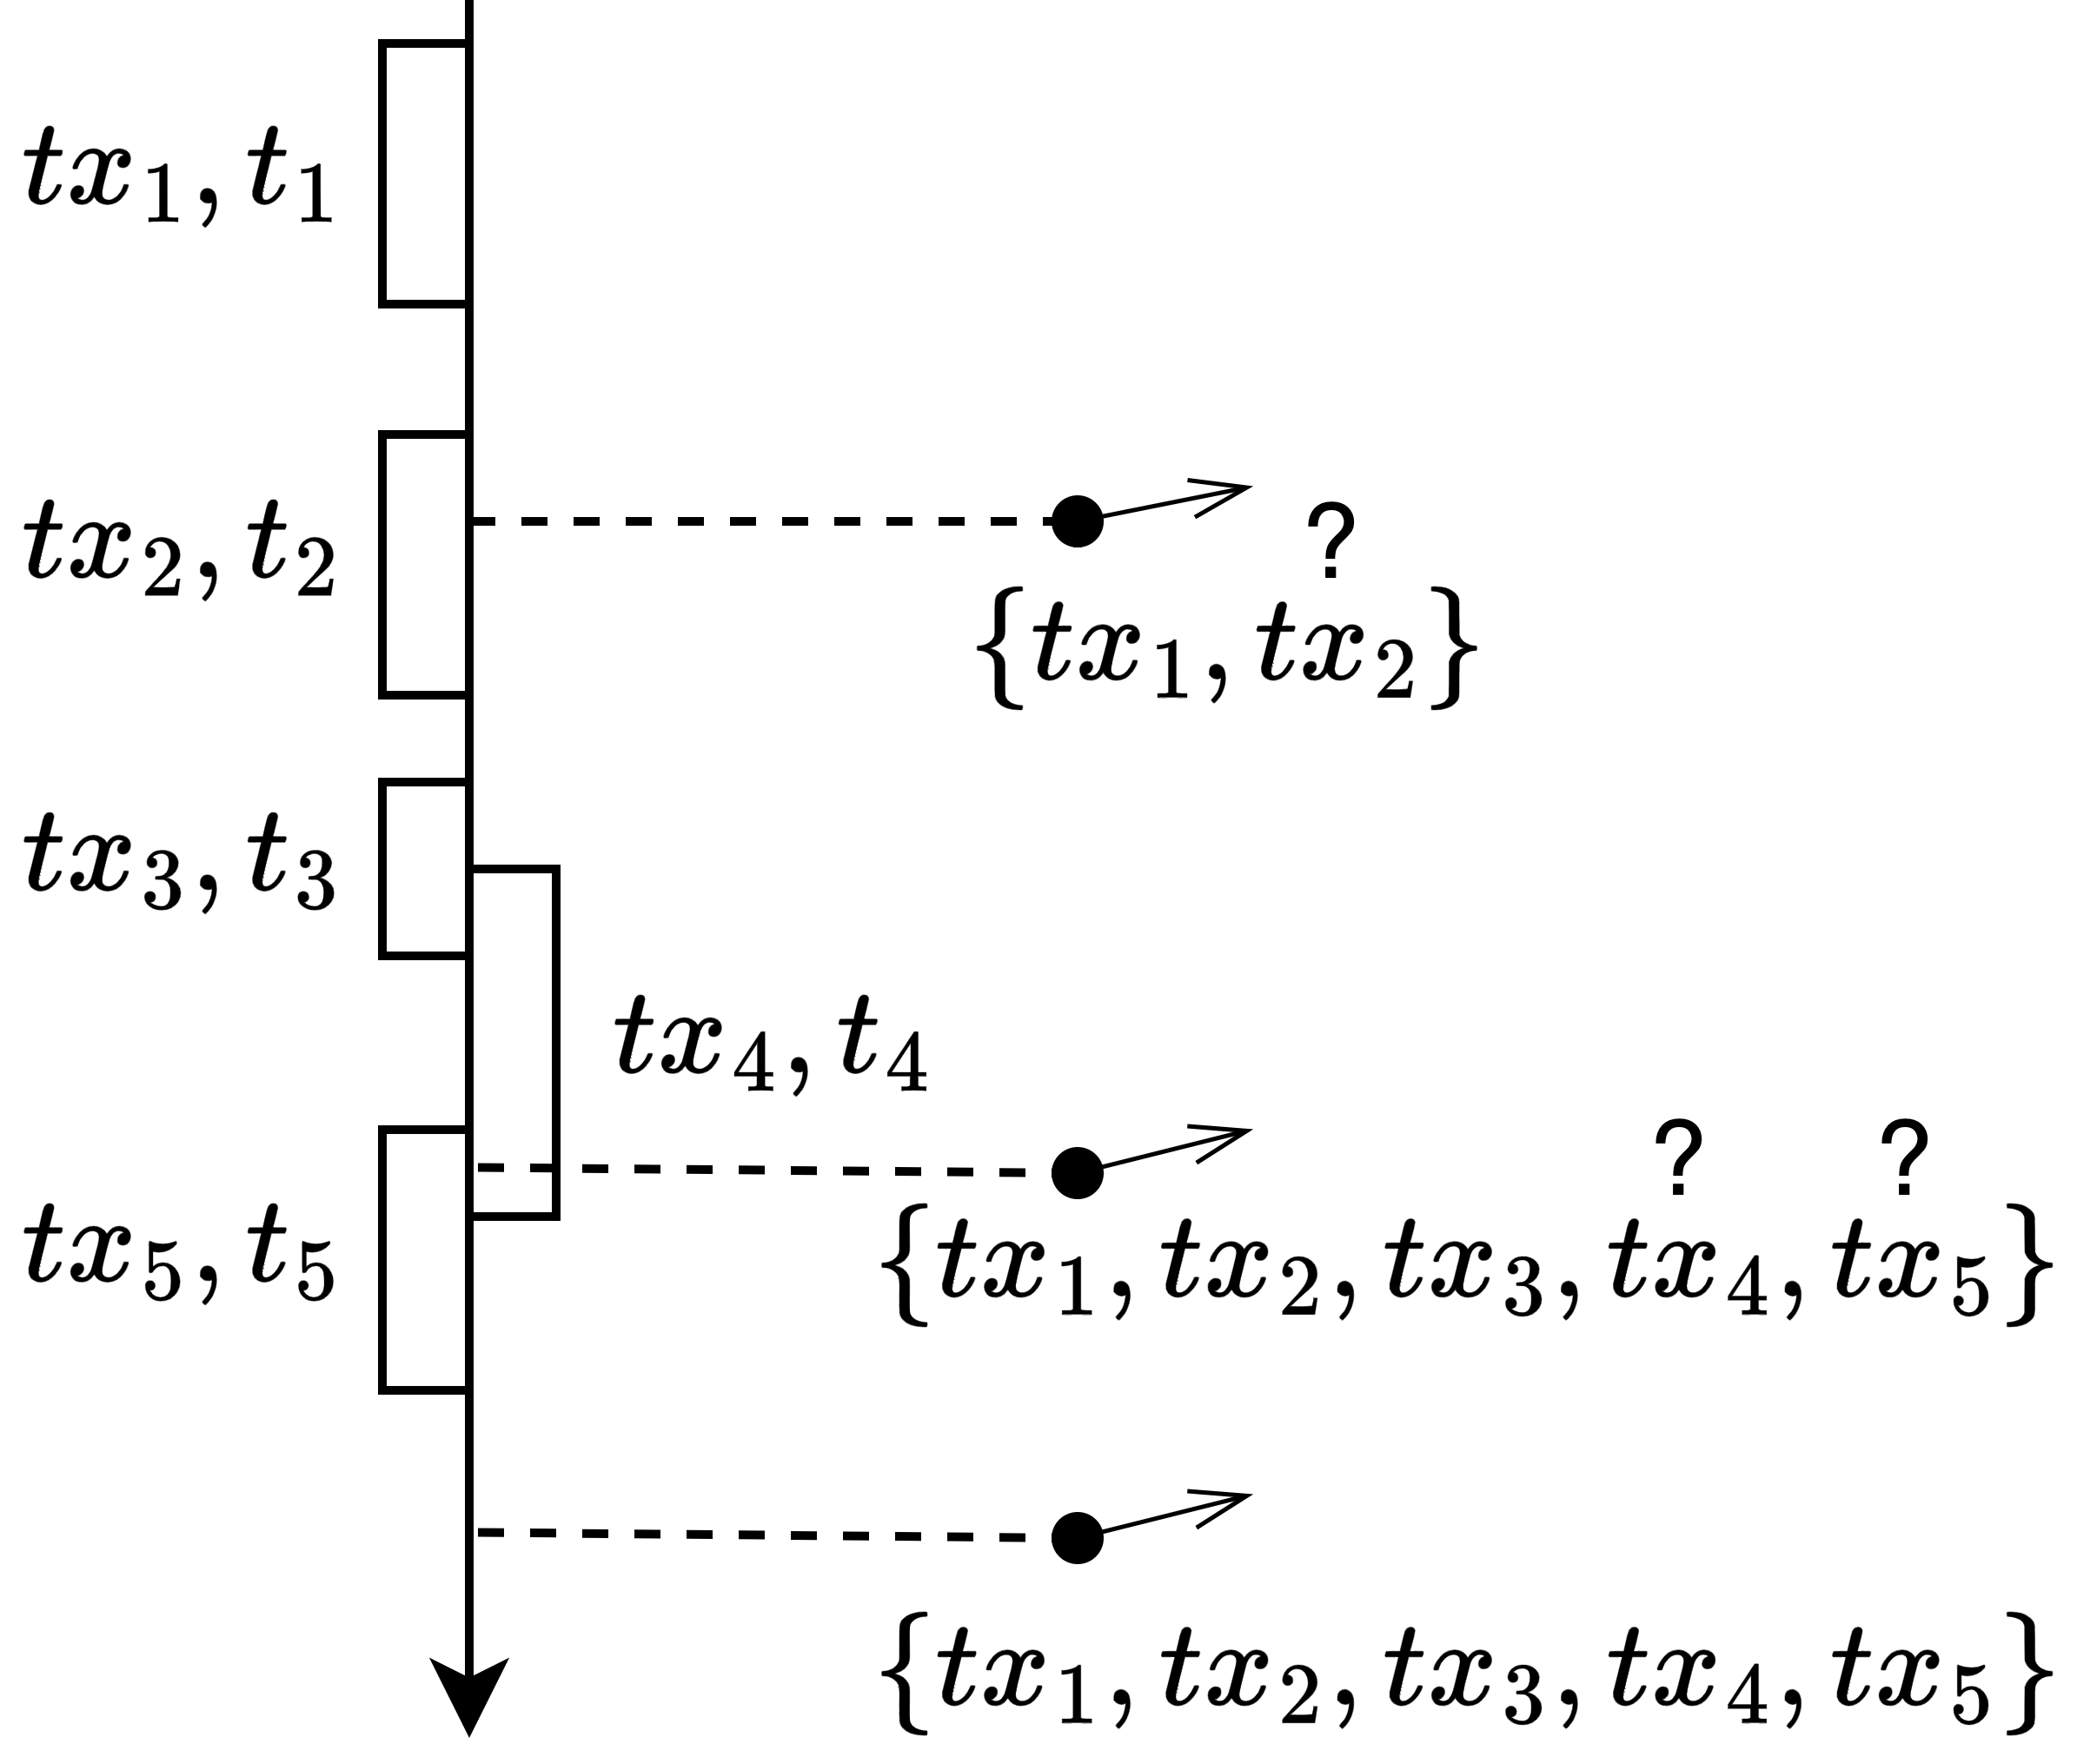
\includegraphics[width=\textwidth]{images/tx_flow.png}
      \vspace*{-3mm}
      \captionof{figure}{Example, POD assigning timestamps to transactions}\label{fig:pod-tx-flow}
    \end{center}
  \end{minipage} 
  \quad
  \begin{minipage}{.45\textwidth}
    \begin{center}
    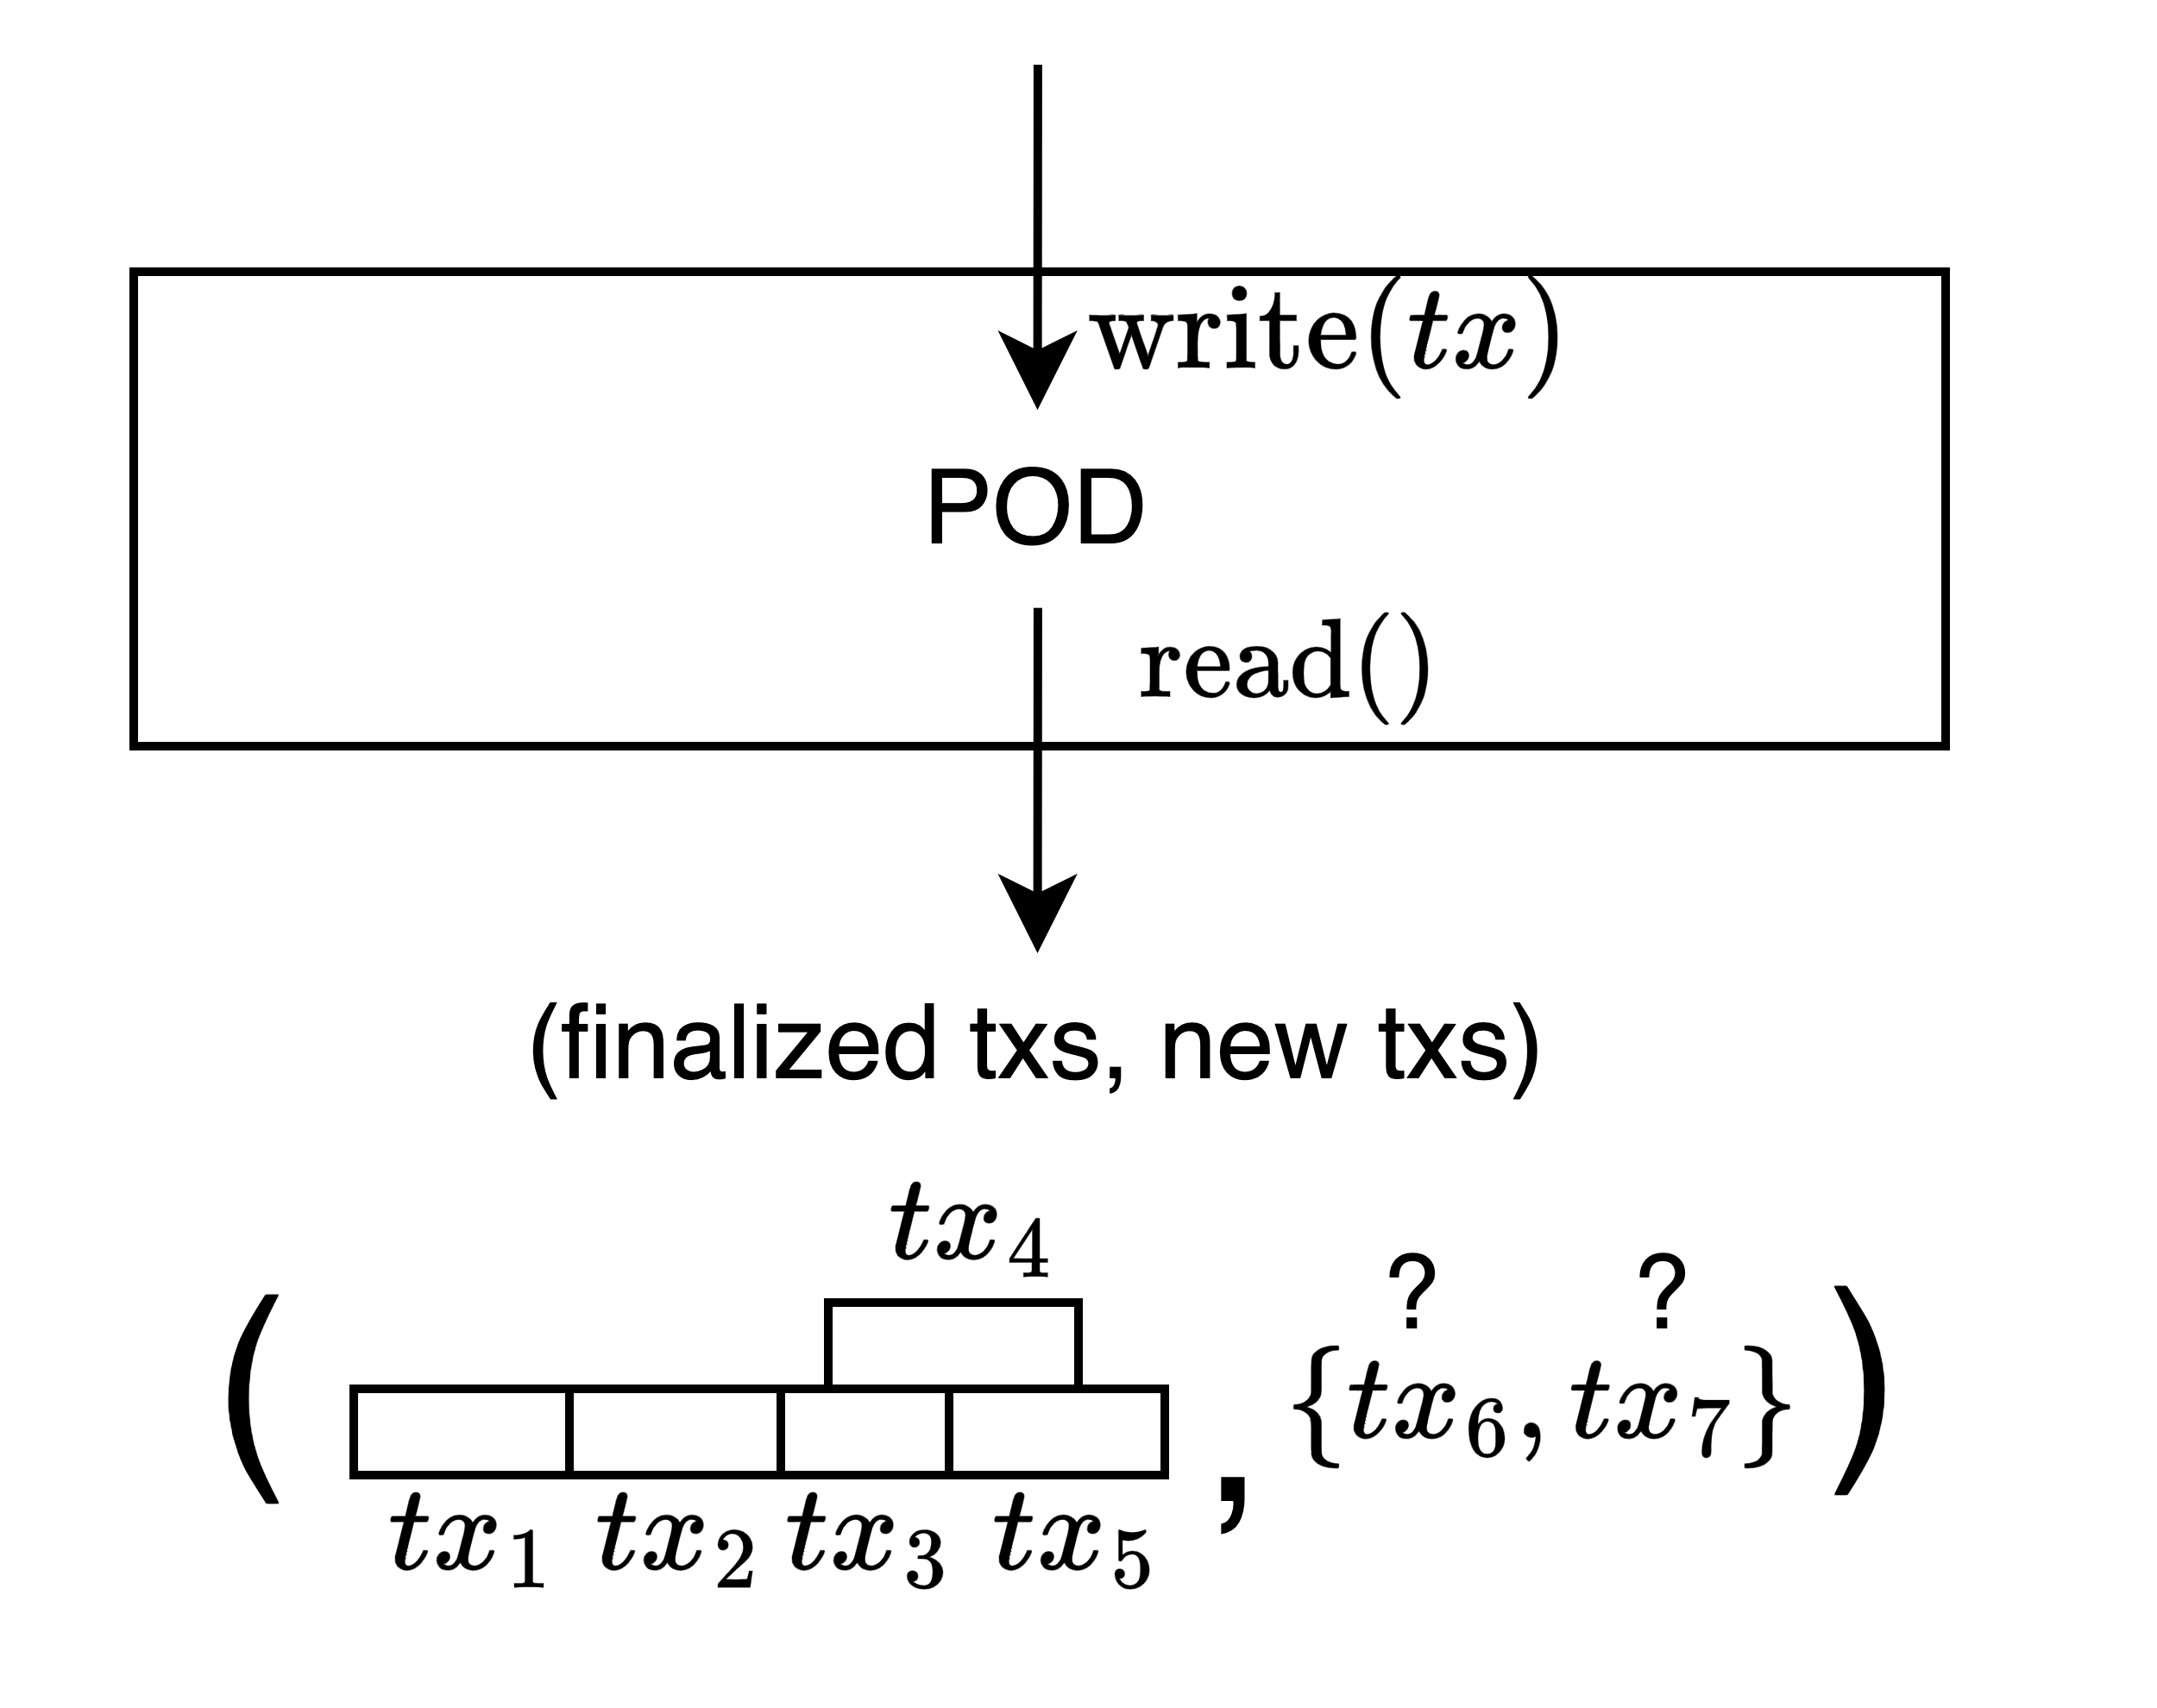
\includegraphics[width=\textwidth]{images/pod-if.png}
    \vspace*{-3mm}
      \captionof{figure}{The interface of POD}\label{fig:pod-if}
    \end{center}
  \end{minipage}


In \Cref{fig:pod-tx-flow} we show an example. The timestamp of $\tx_1$ fluctuates, and transaction $\tx_2$ may or may not be returned by the first read operation.
Similarly, the second read operation may include any subset of $\tx_4, \tx_5$,
but it will include all previously written transactions.
Concurrent transactions, such as $\tx_3$ and $\tx_4$, may be observed by users in any order forever.
Moreover, POD uses the notion of a \emph{past-perfect} timestamp, akin to a `final' block in classical consensus algorithms.
When a timestamp becomes past-perfect, honest users are guaranteed that no more transactions will ever be output with
a timestamp smaller than the past-perfect.
% In the example, $t_5$ is a past-perfect timestamp.    
This is illustrated in \Cref{fig:pod-if}, where the output of the protocol contains
a `finalized' part and an evolving part. 

Currently, the construction works as follows.
Clients write a transaction  by sending it to all replicas in the system.
Replicas can run the code for Certificate Transparency\footnote{\url{https://certificate.transparency.dev/}} to record transactions with timestamps,
with the addition of a Merkle Mountain Range (MMR) data structure, which allows light clients to bloom-filter for inclusion efficiently.
When reading from the system, clients use the mean among the responses from 2/3 of the replicas.
The past-perfection guarantees can be obtained either by separately running an agreement protocol (with timestamps as input, completely decoupled from the observed transactions),
or by having the reading client engage in a two-round protocol with the replicas.

\dotparagraph{Scope}
This proposal includes, but is not limited to, the following items.
\begin{itemize}[left=0pt,itemindent=0pt]
    \item Make POD work in a semi-permissioned model (proof-of-stake–capable, akin to Tendermint~\cite{DBLP:journals/corr/abs-1807-04938}).
    % Our current design works in a permissioned model (akin to HotStuff, Streamlet, and others).
    \item Explore ways to introduce rational arguments to the replicas.
    % We provide resilience and some guarantees in the full Byzantine model, assuming an adversary that controls $f < n/3$ replicas,
    \item Explore the idea of providing `flexible', per-client ordering guarantees, based on local beliefs. Similar techniques have been used to resolve the dilemma between dynamically available and safe-under-asynchrony blockchains~\cite{DBLP:conf/sp/NeuTT21}.
    \item Explore mechanisms to bring the rate of timestamp fluctuation down with time,  so that the system converges to full consensus.
    \item Implement and evaluate POD based on an existing codebase, such as Google's Certificate Transparency implementation\footnote{\url{https://github.com/google/certificate-transparency-go}} or FastPay~\cite{DBLP:conf/aft/BaudetDS20}.
\end{itemize}


\section{Budget}
